\documentclass{beamer}
\usepackage[utf8]{inputenc}
\usepackage{url}
\graphicspath{{./fig/aula3}}
\usepackage{comment}

% Configurando layout para mostrar codigos C++
\usepackage{listings}
\lstset{
  language=HTML,
  basicstyle=\ttfamily\small, 
  keywordstyle=\color{blue}, 
  stringstyle=\color{red}, 
  commentstyle=\color{red}, 
  extendedchars=true, 
  showspaces=false, 
  showstringspaces=false, 
  numbers=left,
  numberstyle=\tiny,
  breaklines=true, 
  backgroundcolor=\color{green!10},
  breakautoindent=true, 
  captionpos=b,
  xleftmargin=0pt,
}


\title{Desenvolvimento Web Básico}
\subtitle{Aula 3}

\usetheme{lucid}
\date{}

\begin{document}
\frame{
 \titlepage
}

\section{Introdução}
\begin{frame}{Recapitulando...}
Nas últimas aulas vimos:
  \begin{enumerate}
   \item Tags HTML;
   \item Elementos básicos HTML;
   \item Folha de estilos;
  \end{enumerate}
\end{frame}
%------------------------------------------------------------------------------------------
\begin{frame}
\frametitle{Roteiro} % Table of contents slide, comment this block out to remove it
\tableofcontents % Throughout your presentation, if you choose to use \section{} and \subsection{} commands, 
%these will automatically be printed on this slide as an overview of your presentation
\end{frame}
%-------------------------------------------------------------------------------
\begin{frame}{Introdução}
\begin{block}{CSS}
CSS é a sigla para o termo em inglês Cascading Style Sheets que, traduzido para o português, significa Folha de Estilo em Cascatas. O CSS é fácil de aprender e entender e é facilmente utilizado com as linguagens de marcação HTML ou XHTML. 
\end{block}
\end{frame}
%-------------------------------------------------------------------------------
\begin{frame}{Introdução}
\begin{block}{História}
CSS foi desenvolvido pelo W3C (World Wide Web Consortium) em 1996, por uma razão bem simples. \\
O HTML não foi projetado para ter tags que ajudariam a formatar a página. \\
Você deveria apenas escrever a marcação para o site.
\end{block}
\end{frame}
%-------------------------------------------------------------------------------
\section{CSS}
\begin{frame}{Sintaxe CSS}
  \begin{center}
    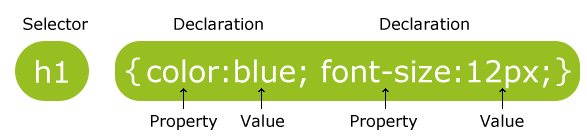
\includegraphics[height=0.25\paperheight]{fig/aula2/css_sintax.png} \\
    \tiny \textbf{Fonte:} \cite{freeman2008use}.
  \end{center}
\end{frame}
%-------------------------------------------------------------------------------
\begin{frame}{Sintaxe CSS}
  \begin{center}
    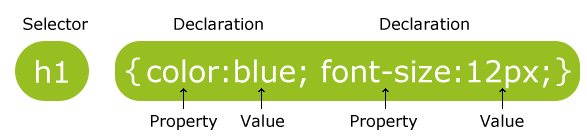
\includegraphics[height=0.25\paperheight]{fig/aula2/css_sintax.png} \\
    \tiny \textbf{Fonte:} \cite{freeman2008use}.
  \end{center}
\end{frame}
%-------------------------------------------------------------------------------
\begin{frame}{Inserindo estilo}
Inserindo um arquivo externo CSS.
  \begin{center}
    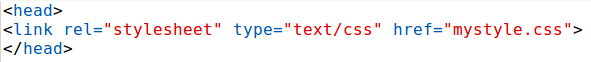
\includegraphics[height=0.12\paperheight]{fig/aula2/external_css.png} \\
    \tiny Link para folha de estilos
  \end{center}
  \begin{center}
    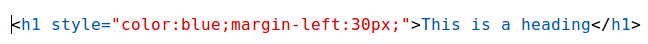
\includegraphics[height=0.08\paperheight]{fig/aula2/estilo_elemento.png} \\
    \tiny Estilo aplicado ao elemento
  \end{center} 
\end{frame}
%-----------------------------------------------------------------------------
\begin{frame}{Inserindo estilo}
Qual seria o resultado se para esta situação?
  \begin{center}
    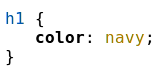
\includegraphics[height=0.2\paperheight]{fig/aula2/h1_css.png} \\
		  \tiny Na folha de estilos mystyle.css
	  \end{center}
	  \begin{center}
		  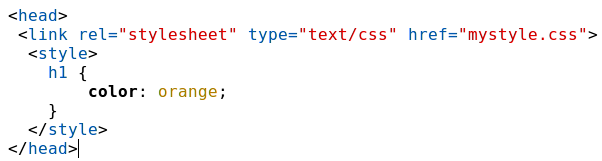
\includegraphics[height=0.3\paperheight]{fig/aula2/h1_html.png} \\
		  \tiny No HTML
	  \end{center}
	  
\end{frame}
%-----------------------------------------------------------------------------
\section{Seletores}
\begin{frame}{Elemento seletor}
  Os elementos Seletores são utilizados para estilizar elementos HTML.\\
  Ele encontra os elementos através do nome, id, classe e atributo.
  \begin{block}{Tipos de seletores*}
    \begin{itemize}
      \item Seletor elementos;
      \item Seletor id;
      \item Seletor classe;
    \end{itemize}
 \tiny *Os seletores apresentados são básicos, existem outros tipos de 
seletores.
  \end{block}
\end{frame}
%---------------------------------------------------------------------------------
\begin{frame}{Seletor Elementos}
Exemplo, seletor de elemento aplicado a $<p>$.
  \begin{center}
    \lstinputlisting{cod/elemento.css}
  \end{center}
\end{frame}
%---------------------------------------------------------------------------------
\begin{frame}{Seletor id}
Exemplo, seletor de elemento aplicado a um elemento com o id ``para1''.
  \begin{center}
    \lstinputlisting{cod/seletor_id.css}
  \end{center}
\end{frame}
%---------------------------------------------------------------------------------
\begin{frame}{Seletor classe}
Exemplo, seletor de elemento aplicado a um elemento definido com a classe ``center''.
  \begin{center}
    \lstinputlisting{cod/seletor_class.css}
  \end{center}
\end{frame}
%---------------------------------------------------------------------------------
\begin{frame}{Seletor classe}
É possível especificar que somente \textbf{um} elemento seja afetado por uma classe:
    \begin{center}
      \lstinputlisting[linerange={1-3}]{cod/seletor_class_element.css}
      \tiny Código HTML
    \end{center}
%   \vspace{0.2cm}
  \begin{center}
    \lstinputlisting[linerange={5-9}]{cod/seletor_class_element.css}
    \tiny Código CSS
  \end{center}
\end{frame}
%---------------------------------------------------------------------------------
\begin{frame}{Seletor classe}
É possível especificar \textbf{mais de uma classe} para um mesmo elemento:
  \begin{center}
    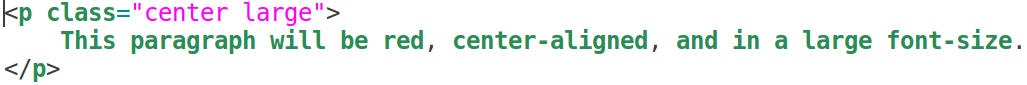
\includegraphics[height=0.1\paperheight]{fig/aula2/css2.png} \\
    \tiny Código HTML
  \end{center}
% 	\vspace{0.2cm}
  \begin{center}
    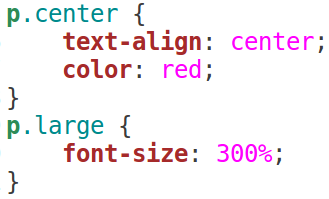
\includegraphics[height=0.2\paperheight]{fig/aula2/css1.png} \\
    \tiny Código CSS
   \end{center}
\end{frame}
%---------------------------------------------------------------------------------
\begin{frame}{Sobre Seletores...}
É possível agrupar seletores que possuem características iguais:
  \begin{columns}
    \begin{column}{0.4\textwidth}
      \begin{center}
	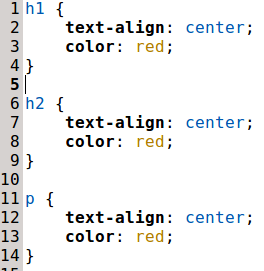
\includegraphics[height=0.45\paperheight]{fig/aula2/seletor_grupo.png} \\
	\tiny Seletores individuais
      \end{center}
    \end{column}
    \begin{column}{0.4\textwidth}
      \begin{center}
	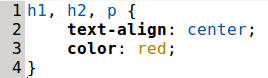
\includegraphics[height=0.15\paperheight]{fig/aula2/seletor_grupo1.png} \\
	\tiny Seletores agrupados
      \end{center}
    \end{column}
   \end{columns}
\end{frame}
%-----------------------------------------------------
\section{Cores e Background}
\begin{frame}{Nome de cores CSS}
	\begin{center}
			\lstinputlisting{cod/colors.css}
			\tiny Para mais cores consulte o \href{https://www.w3schools.com/colors/colors_names.asp}{link}.
		\end{center}
\end{frame}
%----------------------------------------------------------------------------
\begin{frame}{Utilizando Cores CSS}
É possível especificar a cor de vários elementos HTML.
	\begin{center}
		\lstinputlisting[linerange={1-1}]{cod/color_elements.css}
		\tiny Cor de fundo
	\end{center}
% 	\vspace{0.2cm}
	\begin{center}
		\lstinputlisting[linerange={2-2}]{cod/color_elements.css}
		\tiny Cor da fonte
	\end{center}
	\begin{center}
		\lstinputlisting[linerange={3-3}]{cod/color_elements.css}
		\tiny Cor da borda
	\end{center}
\end{frame}
%---------------------------------------------------------------------------------
\begin{frame}{Cores CSS - RGB}
É possível criar muitas cores utilizando RGB (red, green, blue)\\
	\begin{center}
		  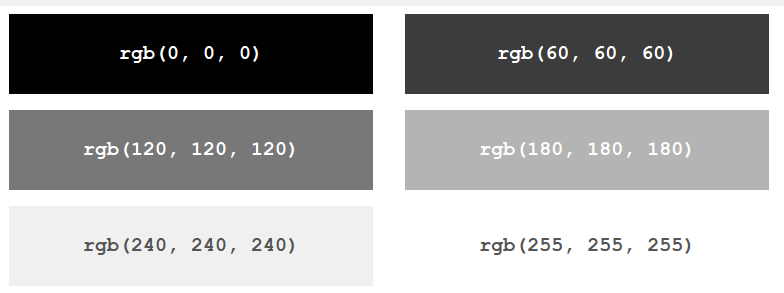
\includegraphics[height=0.4\paperheight]{fig/aula2/rgb.png} \\
		  \tiny Cores rgb.
	  \end{center}
	  \begin{center}
		\lstinputlisting[linerange={4-4}]{cod/color_elements.css}
		\tiny Exemplo de uso RGB
	\end{center}
	  
\end{frame}
%---------------------------------------------------------------------------------
\begin{frame}{Cores CSS - HEX}
É possível criar muitas cores utilizando Hexadecimal \#rrggbb\\
	\begin{center}
		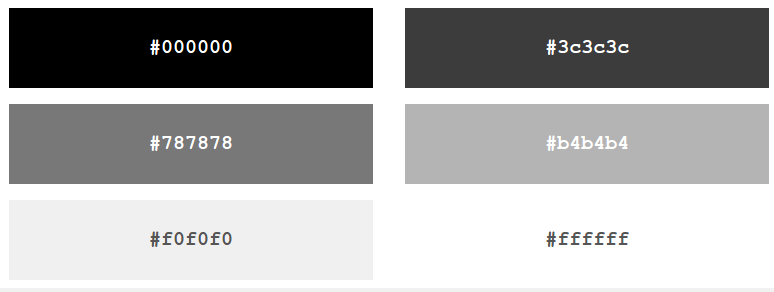
\includegraphics[height=0.4\paperheight]{fig/aula2/hex.png} \\
		\tiny Cores Hexadecimal.
	\end{center}
	\begin{center}
		\lstinputlisting[linerange={5-5}]{cod/color_elements.css}
		\tiny Exemplo de uso Hexadecimal
	\end{center}
	  
\end{frame}
%---------------------------------------------------------------------------------
\begin{frame}{Cores CSS - RGBA}
Precisa de transparência? rgba(\textcolor{red}{Red}, \textcolor{green}{Green}, \textcolor{blue}{Blue}, 
alpha)\\
	\begin{center}
		  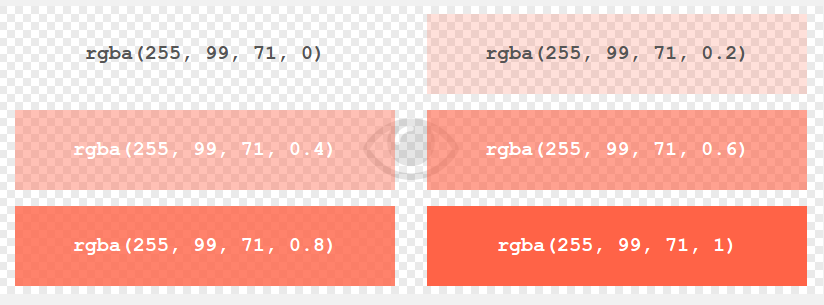
\includegraphics[height=0.4\paperheight]{fig/aula2/rgba.png} \\
		  \tiny Cores Hexadecimal.
	  \end{center}
	  \begin{center}
		\lstinputlisting[linerange={6-6}]{cod/color_elements.css}
		\tiny Exemplo de uso RGBA
	\end{center}
	  
\end{frame}
%---------------------------------------------------------------------------------
\begin{frame}{O poder das Cores CSS}
Colorindo elementos com CSS.\\
Crie uma página colors\_page.html com essa estrutura:
	\begin{center}
	 \lstinputlisting[linerange={21-28}]{cod/colors_page.html}
	\end{center}	  
\end{frame}
%-----------------------------------------------------
\begin{frame}{O poder das Cores CSS}
Acrescente este estilo:
	\begin{center}
	 \lstinputlisting[linerange={5-15}]{cod/colors_page.html}
	\end{center}	  
\end{frame}

%-----------------------------------------------------
\begin{frame}{CSS Background}
Por padrão, uma imagem definida como ``fundo'' de página é repetida. Vejamos o exemplo.\\
Acrescente este comando a página colors\_page.html 
	\begin{center}
	 \lstinputlisting[linerange={16-18}]{cod/colors_page.html}
	\end{center}	 
	A imagem esta disponível no link \href{https://1drv.ms/u/s!AkCRf1UFW3BnjMN39kSRO8ijd5nxLg?e=vfcLWp}{LINK paper.jpg}
\end{frame}
% %---------------------------------------------------
\begin{frame}{CSS Background}
Algumas imagens se repetem horizontalmente ou verticalmente:
Edite o background-image na página colors\_page.html 
	\begin{center}
	 \lstinputlisting[linerange={30-32}]{cod/colors_page.html}
	\end{center}	 
	A imagem esta disponível no link \href{https://1drv.ms/u/s!AkCRf1UFW3BnjMN106yoqqENJ2lZTQ?e=bQpiFu}{LINK gradiente.png}
	
Se a imagem fosse repetida horizontalmente? Como ficaria?
  \begin{center}
	 \lstinputlisting[linerange={33-33}]{cod/colors_page.html}
	 \tiny{Acrescente ao seu código CSS que formata body}
	\end{center}
\end{frame}
%---------------------------------------------------------------------------------
\begin{frame}{CSS Background}
E se não quiser repetição na imagem de fundo?
Edite o background-image na página colors\_page.html 
\begin{center}
	 \lstinputlisting[linerange={36-36}]{cod/colors_page.html}
	 \tiny Acrescente ao seu código CSS que formata body\\ 
	 background-repeat: repeat-y; repete verticalmente
	\end{center}
\end{frame}
% ----------------------------------------------------
\begin{frame}{Background mais opções}

Edite o background-image na página colors\_page.html 
	\begin{center}
	 \lstinputlisting[linerange={34-37}]{cod/colors_page.html}
	\end{center}	 
	A imagem esta disponível no link \href{https://goo.gl/images/aSBzRd}{https://goo.gl/images/aSBzRd}
	
	Coloque a imagem de fundo no canto direito da página, usando o comando abaixo:
\begin{center}
	 \lstinputlisting[linerange={38-38}]{cod/colors_page.html}
	 \tiny Acrescente ao seu código CSS que formata body\\
	\end{center}
\end{frame}
%-----------------------------------------------------
\begin{frame}{CSS Background}
Replique o texto do corpo da página muitas vezes. Role a página.\\

Vamos fixar a imagem no topo da página:
\begin{center}
	 \lstinputlisting[linerange={39-39}]{cod/colors_page.html}
	 \tiny Acrescente ao seu código CSS que formata body\\
	\end{center}
\end{frame}
%-----------------------------------------------------
\begin{frame}{CSS Background}
Adaptando o espaço de texto\\
\begin{center}
	 \lstinputlisting[linerange={42-42}]{cod/colors_page.html}
	 \tiny Acrescente ao seu código CSS que formata body\\
	\end{center}

Utilizando uma forma ``curta'' (\textit{shorthand}) de escrever estilos:
\begin{center}
	 \lstinputlisting[linerange={40-43}]{cod/colors_page.html}
	 \tiny Edite o código CSS que formata body\\
	\end{center}
\end{frame}
%-----------------------------------------------------
\begin{frame}{CSS Background}
Para utilizar a formatação \textit{shorthand}, utlize as especificações na seguinte ordem:
 \begin{itemize}
  \item background-color
  \item background-image
  \item background-repeat
  \item background-attachment
  \item background-position
 \end{itemize}

\end{frame}
%-----------------------------------------------------
\begin{frame}{CSS background - Resumo}
\small
\begin{table}[]
\centering
\begin{tabular}{|l|l|}
\hline
\multicolumn{1}{|c|}{\textbf{Property}} & \multicolumn{1}{c|}{\textbf{Description}} \\ \hline
background & Altera todas as propriedades em uma declaração; \\ \hline
background-attachment & Define se a imagem de fundo é fixa ou não; \\ \hline
background-color & Altera a cor de fundo de um elemento; \\ \hline
background-image & Altera a imagem de fundo de um elemento; \\ \hline
background-position & Define a posição de uma imagem de fundo; \\ \hline
background-repeat & Define se uma imagem de fundo repete. \\ \hline
\end{tabular}
\end{table}
\end{frame}
\begin{comment}
    %-----------------------------------------------------
\section{Bordas}
\begin{frame}{Bordas CSS}
	Propriedades de borda
 \begin{itemize}
  \item \textbf{dotted} - Define uma borda pontilhada
	\item \textbf{dashed} - Define uma borda tracejada
	\item \textbf{solid} - Define uma borda sólido
	\item \textbf{double} - Define uma margem dupla
  \item \textbf{groove} - Define uma borda sulcada 3D. O efeito depende do valor border-color
 \end{itemize}

\end{frame}
%-----------------------------------------------------
\begin{frame}{Bordas CSS}
	Propriedades de borda
 \begin{itemize}
	\item \textbf{ridge} - Define uma borda ridged 3D. O efeito depende do valor border-color
	\item \textbf{inset} - Define uma borda inset 3D. O efeito depende do valor border-color
	\item \textbf{outset} - Define uma borda início 3D. O efeito depende do valor border-color
	\item \textbf{none} - Define sem fronteira
	\item \textbf{hidden} - Define uma borda escondida
 \end{itemize}
\end{frame}
%-----------------------------------------------------
\begin{frame}{Bordas CSS}
Para editar partes da borda:
\begin{itemize}
	\item \textbf{border-top-style:} dotted;
  \item \textbf{border-right-style:} solid;
  \item \textbf{border-bottom-style:} dotted;
  \item \textbf{border-left-style:} solid;
  \item \textbf{border-width:} 20px;
 \end{itemize}
 \tiny Fontes: \cite{wschool2018html, purewal2014learning}
\end{frame}
%-----------------------------------------------------
\begin{frame}{CSS com base no estado}
É possível estilizar elementos com base no estado deles:\\
O CSS abaixo estiliza um link de verde quando não visitado, rosa quando visitado e sem decoração ao passar do mouse.
\begin{center}
		  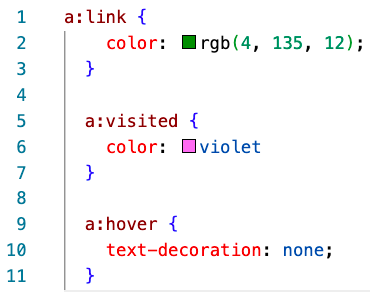
\includegraphics[height=0.4\paperheight]{fig/aula2/css_estado.png} \\
	  \end{center}
 \tiny Fontes: \cite{mdn2023}
\end{frame}

%-----------------------------------------------------
\begin{frame}{CSS Função}
Uma função consiste em chamar o nome de uma uma função e um par de perenteses, entre os parenteses são iformados os parâmetros.\\
No caso da função \textbf{calc()} o desenvolvedor inform que a largura da div deve ser 90\% do bloco onde ela está, menos 30px.\\
\begin{columns}
\begin{column}{0.5\textwidth}
        \begin{center}
		  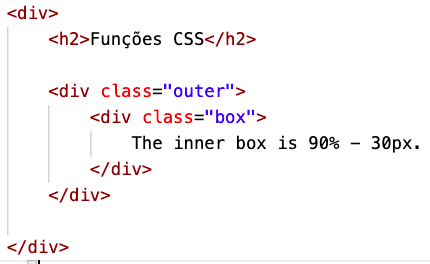
\includegraphics[height=0.4\paperheight]{fig/aula2/layout_html1.png} \\
		  \tiny{Código HTML}
	  \end{center}
   \end{column}
   \begin{column}{0.5\textwidth}
        \begin{center}
		  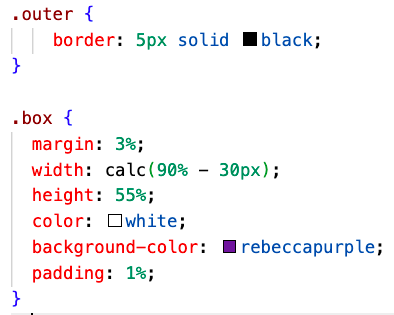
\includegraphics[height=0.4\paperheight]{fig/aula2/layout_css2.png} \\
		  \tiny{Código CSS}
	  \end{center}
	  
   \end{column}
\end{columns}
 \tiny Fontes: \cite{mdn2023}
\end{frame}
%-----------------------------------------------------
\begin{frame}{CSS Função}
Outro exemplo de função é a rotate aplicada a propriedade transform.\\
\begin{columns}
\begin{column}{0.5\textwidth}
        \begin{center}
		  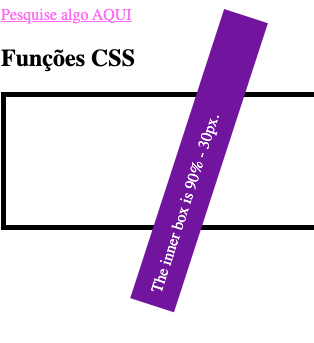
\includegraphics[height=0.4\paperheight]{fig/aula2/layout_html2.png} \\
		  \tiny{Saída do Código HTML}
	  \end{center}
   \end{column}
   \begin{column}{0.5\textwidth}
        \begin{center}
		  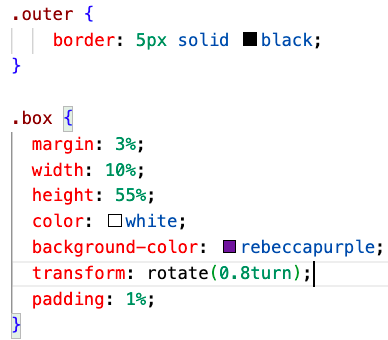
\includegraphics[height=0.4\paperheight]{fig/aula2/layout_css1.png} \\
		  \tiny{Código CSS: Edite o código anterior para width: 20\% e acrescente a propriedade transform.}
	  \end{center}
	  
   \end{column}
\end{columns}
 \tiny Fontes: \cite{mdn2023}
\end{frame}

%-----------------------------------------------------
\begin{frame}{CSS Regras}
Regras CSS são aplicadas com o operador \@. E descrevem formatações CSS que só serão aplicadas dependendo de uma determinada condição.
\begin{columns}
\begin{column}{0.5\textwidth}
        A regra ao lado será aplicada apenas se o monitor que exibe o seu site tiver mais de 30em
   \end{column}
   \begin{column}{0.5\textwidth}
        \begin{center}
		  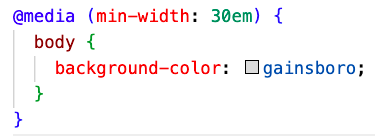
\includegraphics[height=0.2\paperheight]{fig/aula2/layout_css3.png} \\
		  \tiny{Código CSS: Acrescente este código ao CSS anterior.}
	  \end{center}
	  
   \end{column}
\end{columns}
Teste a visualização no modo celular nas opções de "inspecionar" do Chrome.\\
 \tiny Fontes: \cite{mdn2023}
\end{frame}
%-----------------------------------------
\begin{frame}{DOM}
\begin{itemize}
    \item O navegador carrega o HTML e converte o HTML para um DOM (\textit{Document Object Model}). O DOM representa o documento na memória do computador.
    \item O navegador requisita a maioria dos recursos que estão vinculados ao documento HTML, como imagens encorporadas e vídeos, e também, folhas de estilo CSS.
    \item O navegador analisa o CSS encontrado (fetched) e interpreta as diferentes regras por meio dos de seletores, tais como elementos (ex: h1, h2), classes (.myElement), ID (\#myNav), e outros...
    \item Com base nos seletores, o navegador insere as regras de estilização que devem ser aplicadas para cada nó no DOM, e aplica o estilo para os elementos como especificado nas folhas de estilização (este processo intermediário é chamado de render tree ou árvore de renderização).
\end{itemize}
\end{frame}
%---------------------
\begin{frame}{Processamento de página - Esquema}
\begin{center}
		  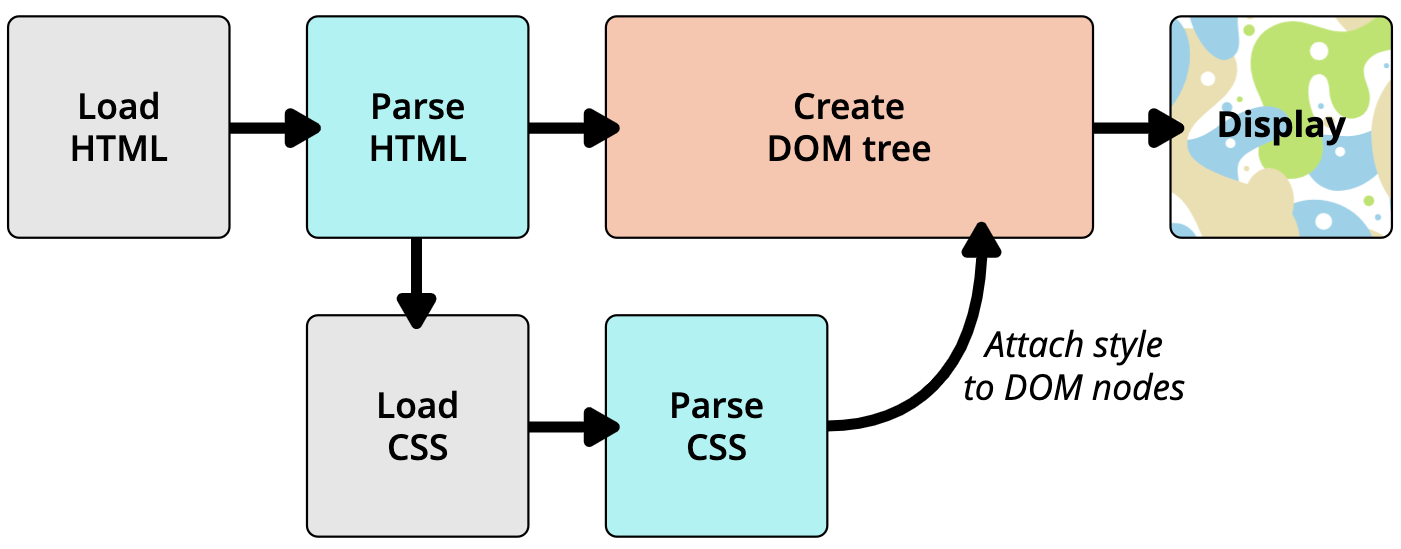
\includegraphics[height=0.45\paperheight]{fig/aula2/dom.png} \\
		   \tiny Fontes: \cite{mdn2023}
	  \end{center}
    
\end{frame}
%-----------------------------------------------------
\begin{frame}{DOM - Exemplo}
\begin{columns}
\begin{column}{0.5\textwidth}
        \begin{center}
		  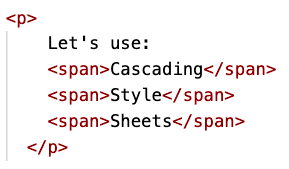
\includegraphics[height=0.4\paperheight]{fig/aula2/dom3.png} \\
		  \tiny{Código HTML}
	  \end{center}
   \end{column}
   \begin{column}{0.5\textwidth}
        \begin{center}
		  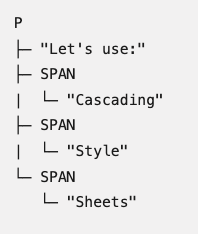
\includegraphics[height=0.4\paperheight]{fig/aula2/dom2.png} \\
		  \tiny{Código CSS}
	  \end{center}
	  
   \end{column}
\end{columns}

\end{frame}
\end{comment}
%-----------------------------------------------------
\section{Atividades}
\begin{frame}{Atividade 1}
Sobre barras de navegação. Vamos utilizar alguns conceitos conhecidos para criar uma barra de navegação 
vertical.
	\begin{center}
		  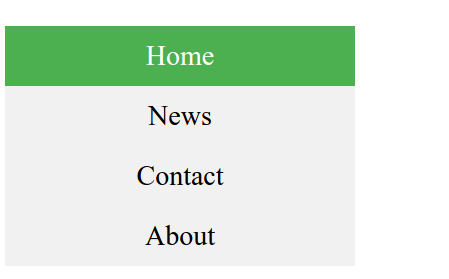
\includegraphics[height=0.4\paperheight]{fig/aula2/aep_1_2.png} \\
	  \end{center}
\end{frame}
%-----------------------------------------------------
\begin{frame}{Atividade 2}
Reproduza a página a seguir utilizando propriedades de borda;
  \begin{center}
    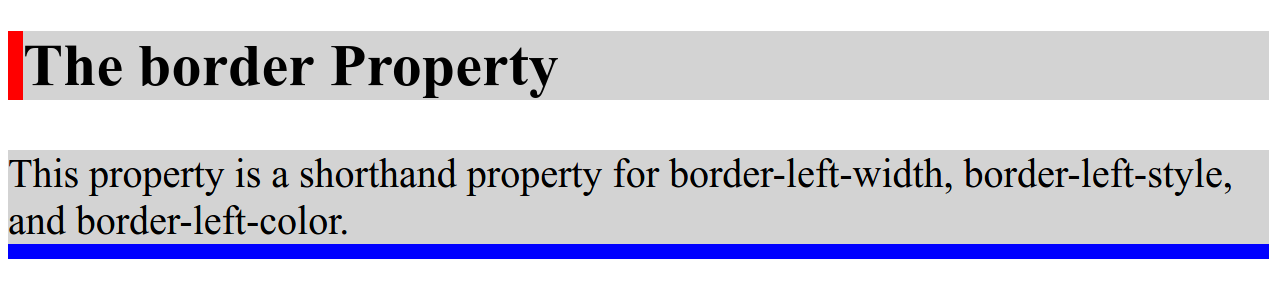
\includegraphics[height=0.2\paperheight]{fig/aula2/AEP_1_1.png} \\
  \end{center}
\end{frame}

%-----------------------------------------------------
\section{Leitura recomendada}
\begin{frame}{Leitura complementar [1]}
 Para mais informações sobre HTML e CSS, leia:\\
 \begin{columns}
   \begin{column}{0.5\textwidth}
    Desenvolvimento de Software II: Introdução ao Desenvolvimento Web com HTML, CSS, JavaScript e PHP \\
     Capítulo 4 - Página 61\\ 
      \cite{miletto2014desenvolvimento}
   \end{column}
   \begin{column}{0.3\textwidth}
    \begin{center}
  
\includegraphics[height=0.45\paperheight]{fig/aula2/milleto2014.jpeg} \\
 \end{center}
   \end{column}
 \end{columns}
\end{frame}

%-----------------------------------------------------
\begin{frame}{Leitura complementar [2]}
 Para mais informações sobre HTML5, leia:\\
 \begin{columns}
   \begin{column}{0.4\textwidth}
     HTML5 - Embarque imediato\\ 
      \cite{flatschart2011html}
   \end{column}
   \begin{column}{0.3\textwidth}
    \begin{center}
  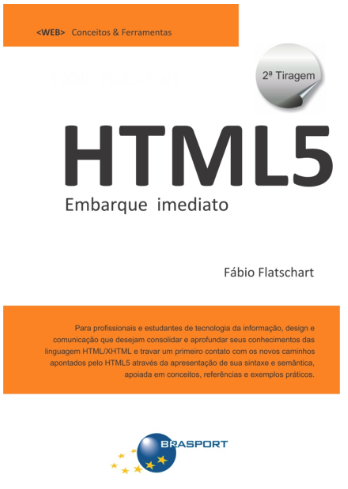
\includegraphics[height=0.5\paperheight]{fig/aula2/flatschart2014html.png} \\
 \end{center}
   \end{column}
 \end{columns}
\end{frame}
%---------------------------------------------------
\section{Referências}
\begin{frame}{Referências}%[allowframebreaks]
\frametitle{Referências}
\small
\begin{center}
\tiny
\bibliographystyle{apalike}
\bibliography{ref_aula}
\end{center}
\end{frame}

\end{document}